\documentclass[aps,%
12pt,%
final,%
oneside,
onecolumn,%
superscriptaddress,%
centertags]{article} %%
\topmargin=10em
\textheight=600pt
\usepackage[english]{babel}
\usepackage[utf8]{inputenc}
\usepackage[colorlinks=true,urlcolor=black,linkcolor=black,filecolor=black,citecolor=black,unicode,pdftex]{hyperref}
\usepackage{supertabular}
\usepackage[pdftex]{graphicx}
\usepackage{amsthm,amssymb, amsmath}
\usepackage{textcomp}
\usepackage[noend]{algorithmic}
\usepackage[ruled]{algorithm}
\selectlanguage{english}

\begin{document}

\begin{titlepage}
\begin{center}

% Title
\textbf{\LARGE Subversion to Git Bridge} \\[1.0cm]
\textbf{\Large Specification Draft} \\[2.0cm]

\textbf{Alexander Kitaev} \\[1.0cm]
\textbf{Dmitry Pavlenko} \\[1.0cm]
\textbf{Marc Strapetz} \\[1.0cm]
\textbf{Semen Vadishev} \\[1.0cm]

\end{center}
\end{titlepage}

\topmargin=-10pt
\setcounter{page}{2}

\newpage
\hrule
\tableofcontents

\newpage
\hrule
\section{Bridge}
\subsection{Subsection 1.}
\subsection{Subsection 2.}

Here goes some text about \emph{Architecture}. %this text is italic

\newpage

Here goes a list\newline % end-of-line marker
\begin{itemize}
	\item Here is the first item
	\item Here is the second one
\end{itemize}

Here is enumerated list\\ %end-of-line marker too
\begin{enumerate}
	\item First item
	\item Second item
\end{enumerate}

And here goes a picture:

\begin{figure}[!h]
\label{arch}
\centering
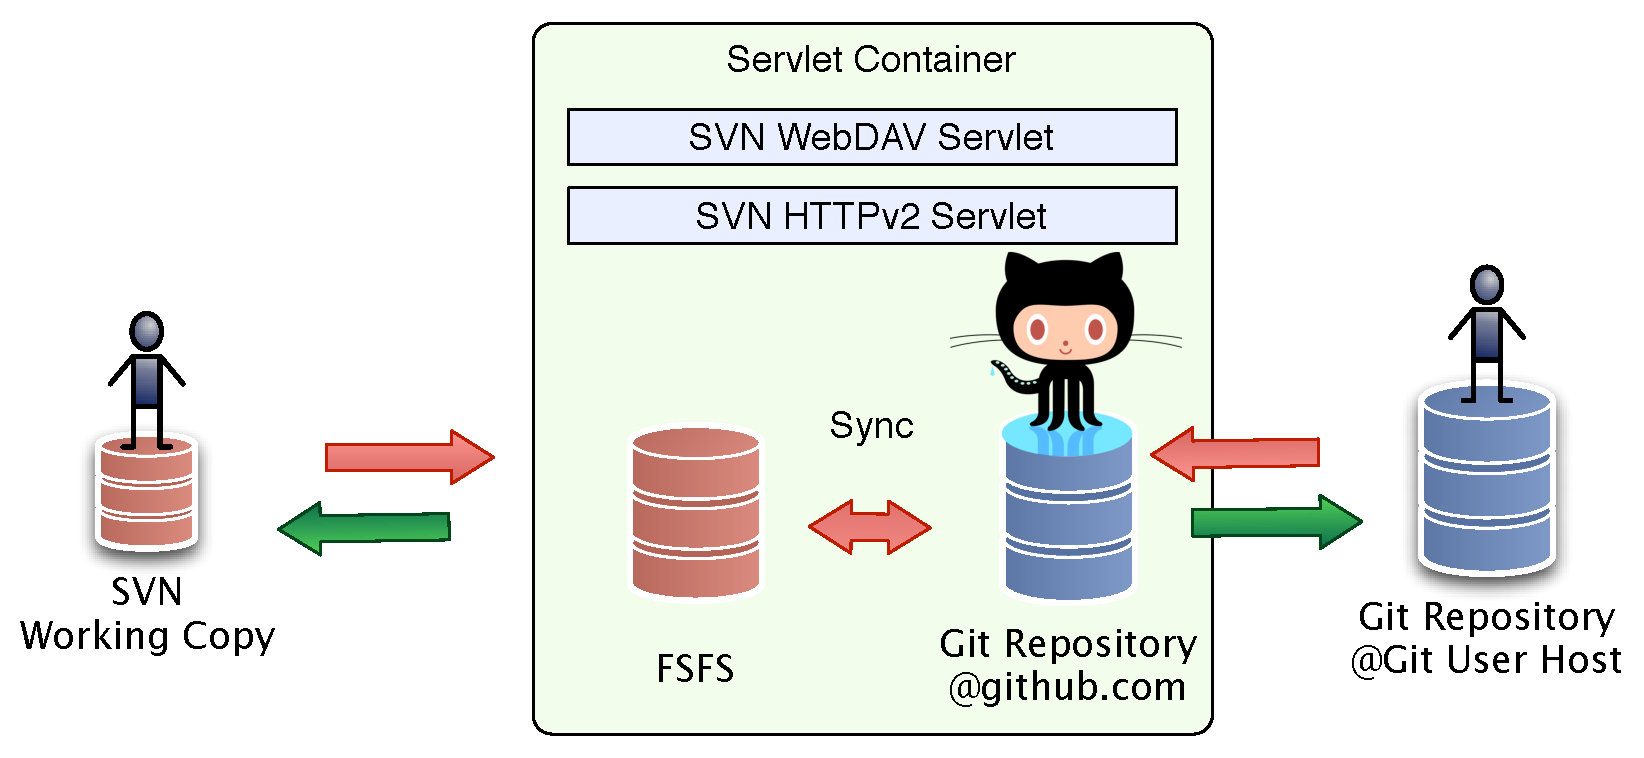
\includegraphics[width=\linewidth]{img/servlet/components_not_that_safe.pdf}
\caption{Architecture.}
\end{figure}

You may use \ref{arch} as a reference to a picture.

\end{document}